\documentclass{article}

\usepackage[dutch]{babel}
\usepackage[margin=3cm]{geometry}
\usepackage{graphicx}
\usepackage{float}
\usepackage{caption}
\usepackage{hyperref}
\usepackage{amsmath}
\usepackage{wrapfig}
\usepackage[parfill]{parskip}

% fonts
\usepackage[T1]{fontenc}
\usepackage{helvet}
\renewcommand{\familydefault}{\sfdefault}

\graphicspath{{img/}}

% theorem environment
\usepackage{amssymb}

\newtheorem{theorem}{Definitie}[section]

\usepackage{enumitem}

\newenvironment{thmenum}
 {\begin{enumerate}[label=\upshape\bfseries(\roman*)]}
 {\end{enumerate}}


% code
\usepackage{minted}
\setminted{frame=single,framesep=3pt,linenos}
\usepackage{upquote}
\usepackage{color}

\begin{document}

\begin{titlepage}
    \author{Tuur Vanhoutte}
    \title{Advanced Programming \& Maths}
\end{titlepage}

\pagenumbering{gobble}
\maketitle
\newpage
\tableofcontents
\newpage

\pagenumbering{arabic}

\section{Basisfuncties in de wiskunde}

\subsection{Functies}

\begin{theorem}[Re"ele functie]
Een re"ele functie is een relatie in $\mathbb{R}$ waarbij elke waarde $x$ hoogstens één beeldwaarde $f(x)$ heeft
\end{theorem}

\begin{figure}[H]
    \centering
    \includegraphics[width=0.5\textwidth]{reele-functie.png}
    \caption{Voorbeelden re"ele functies}
\end{figure}

\begin{theorem}
Voor elke functie geldt: er bestaat een \dots
    \begin{thmenum}
        \item \dots domein van de functie (domain)
        \item \dots beeld van de functie (range)
        \item \dots functievoorschrift van de functie
    \end{thmenum}
\end{theorem}

\begin{figure}[H]
    \centering
    \includegraphics[width=0.5\textwidth]{functie-domain-range.png}
    \caption{Domein, bereik, functievoorschrift}
\end{figure}

$f: \mathbf{domein} \rightarrow \mathbf{bereik}: x \rightarrow y = f(x)$

$f: \mathbb{R} \rightarrow \mathbb{R} : x \rightarrow y = x^3 - 4x$

\begin{theorem}
    Elke functie kan nulpunten hebben.
\end{theorem}

\begin{figure}[H]
    \centering
    \includegraphics[width=0.5\textwidth]{functie-nulpunten.png}
    \caption{$y=-x^3 + 4x$}
\end{figure}

Verloop van een functie wordt via een tekenschema verduidelijkt:

\begin{figure}[H]
    \centering
    \includegraphics[width=0.5\textwidth]{functie-tekenschema.png}
    \caption{Tekenschema}
\end{figure}

\subsection{Veelterm en veeltermfuncties}

\begin{theorem}[Veelterm]
\begin{equation}
    \begin{aligned}
        A(x) = a_nx^n + a_{n-1}x^{n-1} + a_{n-2}x^{n-2} + ... + a_{2}x^{2} + a_1x + a_0\\
        (a_n,a_{n-1},...,a_2,a_1,a_0 \in \mathbb{R})
    \end{aligned}
\end{equation}

\end{theorem}

\begin{theorem}[Veeltermfunctie]
\begin{equation}
    \begin{aligned}
        f(x) = a_nx^n + a_{n-1}x^{n-1} + a_{n-2}x^{n-2} + ... + a_{2}x^{2} + a_1x + a_0\\
        Graad\ van\ veelterm = n\ als\ a_n \neq 0
    \end{aligned}
\end{equation}
\end{theorem}

\subsection{Bijzondere veeltermfuncties}

\begin{itemize}
    \item Constante functie: $f(x) = 4$
    \item Lineaire functie: $f(x) = 4$
    \item Tweedegraadsfunctie: $f(x) = 3x^2 + 2x + 1$
    \item Derdegraadsfunctie: $f(x) = 5x^3 - 3x^2 + 2x - 1$
    \item Exponenti"ele functie: $f(x) = 2^x$
    \item Logaritmische functie: $(fx) = log_2(x)$
\end{itemize}

\subsubsection{Constante functie}

\begin{figure}[H]
    \centering
    \includegraphics[width=0.3\textwidth]{functie-constant.png}
    \caption{$y=4$}
\end{figure}

\subsubsection{Lineaire functie}

\begin{theorem}[Lineaire functie]
    \begin{equation}
        f(x) = ax + b
    \end{equation}


Voorbeeld: $f(x) = 3x + 6$
\end{theorem}

\begin{itemize}
    \item Betekenis van a: de richtingsco"effici"ent (rico)
    \item Betekenis van b: het snijpunt met de y-as
    \item Nulpunt: $f(x) = 0 \\ \Leftrightarrow 3x + 6 = 0 \\ \Leftrightarrow 3x = -6  \\ \Leftrightarrow x = -2$
\end{itemize}

\begin{figure}[H]
    \centering
    \includegraphics[width=0.3\textwidth]{functie-lineair2.png}
    \caption{Meerdere evenwijdige lineaire functies}
\end{figure}

Evenwijdige rechten als: als $a_1 = a_2$

Loodrechte rechten als: als $a_1 \cdot a_2 = -1$

\subsubsection{Tweedegraadsfunctie}

\begin{theorem}
\begin{equation}
    \begin{aligned}
        f(x) = ax^2 + bx + c,\\
        (a \neq 0)
    \end{aligned}
\end{equation}


\end{theorem}

\begin{figure}[H]
    \centering
    \includegraphics[width=0.2\textwidth]{functie-2degraad.png}
    \caption{$f(x) = x^2 - 2x - 3$}
\end{figure}

\begin{itemize}
    \item Betekenis van a: positief $\Rightarrow$ dalparabool, negatief $\Rightarrow$ bergparabool
    \item Nulpunten: via de discriminant berekenen:
\end{itemize}

\begin{theorem}[Discriminant]
Bij een tweedegraadsvergelijking is de discriminant:

\begin{equation}
    D = b^2 - 4ac
\end{equation}
\end{theorem}

\begin{itemize}
    \item Geval 1: $D > 0 \Rightarrow$ de functie heeft 2 nulpunten
    \item Geval 2: $D = 0 \Rightarrow$ de functie heeft 1 nulpunt
    \item Geval 3: $D < 0 \Rightarrow$ de functie heeft géén nulpunten
\end{itemize}

\begin{figure}[H]
    \centering
    \includegraphics[width=0.4\textwidth]{functie-2degraad3.png}
    \includegraphics[width=0.3\textwidth]{functie-2degraad2.png}
    \caption{De discriminant toont de nulpunten}
\end{figure}

\textbf{Nulpunten berekenen:} 

\begin{equation}
    x_{1,2} = \frac{-b \pm \sqrt{D}}{2a}
\end{equation}

\begin{figure}[H]
    \centering
    \includegraphics[width=0.5\textwidth]{functie-2degraad4.png}
    \caption{Symmetrieas: $x = \frac{-b}{2a}$}
\end{figure}

Voorbeeld: 

\begin{figure}[H]
    \centering
    \includegraphics[width=0.5\textwidth]{functie-2degraad5.png}
    \caption{$y = x^2 - 6x + 8$}
\end{figure}

\subsubsection{Derdegraadsfunctie}

\begin{theorem}[Derdegraadsfunctie]
\begin{equation}
    \begin{aligned}
        f(x) = ax^3 + bx^2 + cx + d
        (a \neq 0)
    \end{aligned}
\end{equation}


\end{theorem}

\subsubsection{Exponenti"ele functie}

\begin{theorem}[Exponenti"ele functie]
\begin{equation}
    f(x) = a^{g(x)}
\end{equation}

Met grondtal $a \in \mathbb{R}_0^+ \backslash \{1\}$
\end{theorem}

\begin{figure}[H]
    \centering
    \includegraphics[width=0.3\textwidth]{functie-exponentieel.png}
    \includegraphics[width=0.3\textwidth]{functie-exponentieel2.png}
\end{figure}


\begin{itemize}
    \item Betekenis van a: groeifactor
    \item Wanneer stijgend? 
    \item Wanneer dalend? 
    \item Nulpunten: 
    \item Vaststelling beeld functie
\end{itemize}



\begin{theorem}[Constante van Euler]

\begin{equation}
    \begin{aligned}
        e \approx 2.718281828\dots
    \end{aligned}
\end{equation}

$f(x) = e^x$ is een bijzondere exponenti"ele functie
\end{theorem}

\begin{figure}[H]
    \centering
    \includegraphics[width=0.5\textwidth]{functie-exponentieel3.png}
    \caption{Verschil tussen $2^x$, $3^x$ en $e^x$}
\end{figure}

\section{Exponenti"ele verbanden in data}

\subsection{Lineaire groei}

Kenmerkend:

\begin{itemize}
    \item Per tijdseenheid wordt hetzelfde getal \textbf{opgeteld}
    \item Grafiek is een rechte
    \item Algemene formule (N = aantal, t = tijd, b: beginhoeveelheid): 
    \begin{equation}
        N = a\cdot t + b
    \end{equation}
\end{itemize}

\begin{figure}[H]
    \centering
    \includegraphics[width=0.5\textwidth]{lineaire-groei.png}
    \caption{Lineaire groei}
\end{figure}

\subsection{Exponenti"ele groei}

Kenmerkend: 

\begin{itemize}
    \item Per tijdseenheid wordt de hoeveelheid met hetzelfde getal \textbf{vermenigvuldigd}
    \item Grafiek is een exponenti"ele functie
    \item \textbf{Algemene formule:} 
    \begin{equation}
        N = b \cdot g^t
    \end{equation}
\end{itemize}

\begin{figure}[H]
    \centering
    \includegraphics[width=0.5\textwidth]{exponentiele-groei.png}
    \caption{Exponenti"ele groei}
\end{figure}

\begin{figure}[H]
    \centering
    \includegraphics[width=0.5\textwidth]{voorbeeld-groei.png}
    \caption{Voorbeeld exponenti"ele groei met groeifactor $\approx 1.22$}
\end{figure}


\subsection{Van groeipercentage naar groeifactor}

De toename/afname wordt vaak ook procentueel uitgedrukt

\begin{itemize}
    \item Een jaarlijkse toename van $14.6\%$
    \item Een jaarlijkse afname van $14.6\%$
\end{itemize}

\begin{theorem}[Groeifactor]
De groeifactor is de factor die per tijdseenheid wordt vermenigvuldigd met de vorige waarde.
\end{theorem}

\subsubsection{Percentage naar factor}

\begin{equation}
g = \frac{p + 100}{100}\%
\end{equation} 

\begin{figure}[H]
    \centering
    \includegraphics[width=0.5\textwidth]{percentage-naar-factor.png}
    \caption{Van groeipercentage naar groeifactor}
\end{figure}


\subsubsection{Factor naar percentage}

\begin{figure}[H]
    \centering
    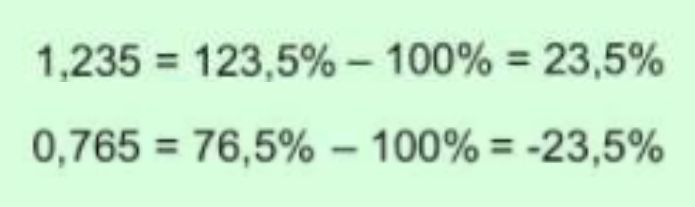
\includegraphics[width=0.35\textwidth]{factor-naar-percentage.png}
    \caption{Van groeifactor naar groeipercentage}
\end{figure}

\begin{figure}[H]
    \centering
    \includegraphics[width=0.5\textwidth]{groeifactoren.png}
    \caption{Let op: hier gebeuren vaak fouten bij het omrekenen}
\end{figure}

\subsection{Voorbeeld}

Een hoeveelheid groeit exponentieel. Na 5u is $N = 82$ en na 12u is $N = 246$.

Stel de formule van N op.

\textbf{Oplossing}

\begin{equation}
N = b \cdot g^t
\end{equation}

\underline{Stap 1: groeifactor berekenen per tijdseenheid:}

\begin{center}
$$
\left.
    \begin{array}{lll}
        \text{Na 5u}  & \rightarrow & N = 82 \\
        \text{Na 12u} & \rightarrow & N = 246 \\
    \end{array}
\right \} \Delta = 7u \rightarrow 164
$$


Groeifactor voor 7 uren: $\frac{246}{82} = 3$

Groeifactor voor 1 uur: $3^{1/7} \approx 1.170$
\end{center}

\underline{Stap 2: 1 punt nemen waarvan we N weten:}

\begin{center}

Gekozen punt: $(5, 82)$

$82 = b \cdot (1.170)^5$

$\Leftrightarrow b = \frac{82}{1.170}^5 \approx 37$

$\Leftrightarrow N = 37 \cdot 1.170^t$
\end{center}

\subsection{Belangrijke maten voor exponenti"ele toename}


\begin{theorem}[Verdubbelingstijd]
De verdubbelingstijd is de nodige tijd tot de hoeveelheid verdubbeld is.

De verdubbelingstijd $t$ kan je berekenen met:
\begin{equation}
g^t = 2
\end{equation}
\end{theorem}

\textbf{Oefening}

De populatie neemt toe met $8.3\%$ per jaar. Bereken de verdubbelingstijd:

\begin{center}
$g^t = 2$

$\Leftrightarrow (1.083)^t = 2$

$\Leftrightarrow \log(1.083^t) = \log(2)$

$\Leftrightarrow t \cdot \log(1.083) = \log(2)$

$\Leftrightarrow t = \frac{\log(2)}{\log(1.083)}$

$\Leftrightarrow t = 8.69\ jaar$

\end{center}


\begin{theorem}[Halveringstijd]
De halveringstijd is de nodige tijd tot de hoeveelheid gehalveerd is.

De halveringstijd $t$ kan je berekenen met:
\begin{equation}
g^t = 1/2
\end{equation}
\end{theorem}

\subsubsection{Oefening: Combinatie van groeifactoren?}

Een hoeveelheid neemt eerst 5 jaar lang met vast percentage (*) toe, 
om daarna nog 3 jaar met 10\% per jaar toe te nemen. Na 8 jaar is
de totale hoeveelheid verdubbeld.

(*) Bereken het jaarlijkse groeipercentage in de eerste 5 jaren.

\textbf{Oplossing}

We weten:

\begin{itemize}
    \item Eerste 5 jaar: toename met vast percentage
    \item Volgende 3 jaar: toename met 10\% (= factor van 1.1)
    \item Na 8 jaar: hoeveelheid verdubbeld (= factor van 2)
\end{itemize}

\begin{center}
$g^5 \cdot 1.1^3 = 2$

We moeten $g$ vinden:

$\Leftrightarrow g^5 = \frac{2}{1.1^3}$

$\Leftrightarrow g = \sqrt[5]{\frac{2}{1.1^3}}$
\end{center}

\section{Belangrijke functies met betrekking tot machine learning}

\subsection{Logistische groei}

\subsubsection{Voorbeeld}

Startsituatie: een bos (bv $\text{10km}^2$) waarin een konijnenepidemie uitbreekt.
Boswachter houdt de populatie van de konijnen bij. Wat stelt hij vast?

De groei van de populatie verloopt volgens een typisch patroon (niet exponentieel):

\begin{figure}[H]
    \centering
    \includegraphics[width=0.5\textwidth]{logistische-groei-vs-exponentieel.png}
    \caption{De rode lijn is de bovengrens}
\end{figure}

\subsubsection{De groei}

= de mate van toename

\begin{itemize}
    \item Hangt af van hoeveel er al zijn tegenover hoeveel er nog bij kunnen
    \item Heel sterke verandering bij start, op het einde heel kleine verandering
    \item Hangt dus ook af van de tijd
\end{itemize}

\begin{theorem}[De logistische groei]
De logistische groei is de mate van toename, afhankelijk van hoeveel er nog bij kan en hoeveel er al is

\begin{equation}
    \frac{\text{Hoeveel er nog bij kan}}{\text{Hoeveel er al is}} = B \cdot g^t
\end{equation}

\begin{itemize}
    \item t = de tijd,
    \item B en g = constanten
\end{itemize}


\end{theorem}

\subsubsection{Functievoorschrift}

\begin{equation}
y = \frac{G}{1 + B\cdot g^t}
\end{equation}

\begin{itemize}
    \item t = de tijd
    \item B en constanten
    \item G = bovengrens
\end{itemize}

\begin{figure}[H]
    \centering
    \includegraphics[width=0.5\textwidth]{logistische-groei.png}
    \caption{Grafiek logistische groei met G = 800}
\end{figure}

\subsubsection{Voorbeeld}

Het aantal vissen in een meer is gegeven door:

\begin{center}
    $N = \frac{2500}{1 + 5.5 \cdot 0.74^t}$
\end{center}

waarbij N = aantal vissen, t = tijd

\textbf{Beredeneer}: Wanneer bereiken we het 'verzadigingsniveau'

Als t heel groot is:

\begin{itemize}
    \item Dan wordt $0.74^t \approx 0$
    \item Dan wordt $5.5 \cdot 0.74^t \approx 0$
    \item Dan wordt $N \approx 2500$
    \item $\Rightarrow$ Het meer is `verzadigd'
\end{itemize}

\subsubsection{Algemene wiskundige notatie van een logistische functie}

\begin{theorem}[Logistische functie]
De wiskundige notatie voor een logistische functie is:

\begin{equation}
    f(x) = \frac{c}{1 + a\cdot b^x}
\end{equation}

met a,b,c constanten waarbij de constante c de belangrijkste is:

c drukt uit wat de maximumwaarde kan zijn
\end{theorem}

\begin{figure}[H]
    \centering
    \includegraphics[width=0.5\textwidth]{logistische-functie-wiskundig.png}
\end{figure}

\subsection{Regression analysis}

Regressieanalyse:

\begin{itemize}
    \item Is er een (voorspellend) verband tussen 2 variabelen
    \item Heeft de ene variabele een invloed op de andere variabele
\end{itemize}

\begin{figure}[H]
    \centering
    \includegraphics[width=0.5\textwidth]{regressie.png}
    \caption{Regressieanalyse}
\end{figure}

\begin{figure}[H]
    \centering
    \includegraphics[width=0.5\textwidth]{regressie2.png}
    \caption{Lineaire vs niet-lineaire samenhang}
\end{figure}


\subsubsection{Lineair regressiemodel}

Enkelvoudige vorm: 

\begin{itemize}
    \item 1 inputwaarde x
    \item via lineaire functie $h_{\theta}(x) = \theta_0 + \theta_1x$
\end{itemize}

\begin{figure}[H]
    \centering
    \includegraphics[width=0.3\textwidth]{lineair-regressiemodel.png}
\end{figure}

\begin{itemize}
    \item Aan de hand van de opgestelde functie doe je een voorspelling
    \item \textbf{Doel:} een zo goed mogelijke lineaire functie opstellen
    \item $\Rightarrow$ zoektocht naar de beste $\theta_0$ en $\theta_1$
\end{itemize}


\subsubsection{Logistisch regressiemodel}

Logistische regressie = \textbf{Classificatie-algoritme}

Zoeken naar een model dat uitkomst (2 mogelijkheden) voorspelt mbv inputwaardes.
Elke inputwaarde heeft een zeker belang (gewicht).

\begin{figure}[H]
    \centering
    \includegraphics[width=0.5\textwidth]{regressiemodel.png}
    \caption{3 inputs met elk een bepaald gewicht, die een uitkomst zoekt (2 mogelijkheden)}
\end{figure}

Vereenvoudiging:  

\begin{itemize}
    \item 1 inputwaarde x
    \item Logistische functie $p = \frac{1}{1 + e^{-(b_0+b_1x)}}$
\end{itemize}

Uitkomst:

\begin{itemize}
    \item de persoon slaagt als $h_{\theta}(x) \geq 0.5$
    \item de persoon slaagt niet als $h_{\theta}(x) < 0.5$
\end{itemize}

\begin{figure}[H]
    \centering
    \includegraphics[width=0.3\textwidth]{logistisch-regressiemodel.png}
    \caption{1 inputwaarde x, met twee  uitkomsten}
\end{figure}

\subsubsection{Lineair vs logistisch regressiemodel}

\begin{figure}[H]
    \centering
    \includegraphics[width=0.5\textwidth]{lineair-vs-logistisch-regression-model.png}
    \caption{Hoe dichter p tegen 1, hoe zekerder het model is}
\end{figure}

Welk model gaat het snelst naar 0 en 1? 

\begin{itemize}
    \item Het logistische model
    \item Daarom is het logistische model beter voor classificate: je splitst de groep op in 2
\end{itemize}

\subsubsection{Meerdere inputfactoren}

Zelfde redenering:

\begin{itemize}
    \item Meerdere inputwaardes $x_1, x_2, \dots$
    \item Gebruik $\theta_0 + \theta_1x_1 + \theta_2x_2 + \dots$
\end{itemize}

\begin{figure}[H]
    \centering
    \includegraphics[width=0.3\textwidth]{logistische-regressie-meerdere-inputfactoren.png}
    \caption{Regressiemodel met meerdere inputfactoren}
\end{figure}


\subsection{Softmax functie}

Doelstelling:

\begin{itemize}
    \item Model dat in staat is om data te gaan categoriseren
    \item Hoe?
    \begin{itemize}
        \item $\Rightarrow$ Met behulp van verschillende inputvariabelen en bijhorende parameters 
    \end{itemize}
\end{itemize}

\begin{figure}[H]
    \centering
    \includegraphics[width=0.35\textwidth]{softmax.png}
    \includegraphics[width=0.4\textwidth]{softmax2.png}
    \caption{Categoriseren met de softmax functie}
\end{figure}

\subsubsection{Kansen}

Kans dat de toestand tot groep A behoort:

\begin{itemize}
    \item $\theta_{A,0} + \theta_{A,1}x_1 + \theta_{A,2}x_2$
    \item Voorbeeld: $0.01 + 0.1x_1 + 0.1x_2$
\end{itemize}

Kans dat de toestand tot groep B behoort:

\begin{itemize}
    \item $\theta_{B,0} + \theta_{B,1}x_1 + \theta_{B,2}x_2$
    \item Voorbeeld: $0.1 + 0.2x_1 + 0.2x_2$
\end{itemize}

Kans dat de toestand tot groep C behoort:

\begin{itemize}
    \item $\theta_{C,0} + \theta_{C,1}x_1 + \theta_{C,2}x_2$
    \item Voorbeeld: $0.1 + 0.3x_1 + 0.3x_2$
\end{itemize}

\subsubsection{Model}

Het softmax-model berekent de mate van zekerheid dat een toestand tot een bepaalde categorie behoort.

vb: volgende quotiënt drukt uit hoe zeker hij is dat (z1, z2) tot categorie A behoort:

$\frac{e^{\theta_{A,0} + \theta_{A,1}z_1 + \theta_{A,2}z_2}}{e^{\theta_{A,0} + \theta_{A,1}z_1 + \theta_{A,2}z_2} + e^{\theta_{B,0} + \theta_{B,1}z_1 + \theta_{B,2}z_2} + e^{\theta_{C,0} + \theta_{C,1}z_1 + \theta_{C,2}z_2} }$

(analoog voor categorie B en C: vervang de teller)

\begin{figure}[H]
    \centering
    \includegraphics[width=0.5\textwidth]{softmax-voorbeeld.png}
    \caption{Betekenis: het model is 29\% zeker dat (0.1, 0.5) tot categorie A behoort. Bereken zelf als oefening voor B en C}
\end{figure}

\subsubsection{Wiskundig}

Het gebruikte model wordt via volgende wiskundige formule algemeen beschreven:

\begin{equation}
\frac{e^{x_k}}{\sum_{i=1}^n e^{x_i}}
\end{equation}

waarbij:

\begin{itemize}
    \item $x_k = \theta_{k,0} + \theta_{k,1}x_1 + \theta_{k,2}x_2 + \dots + \theta_{k,m}x_m$
    \item n = aantal groepen
    \item m = het aantal meetcriteria
\end{itemize}

\subsection{Logistic regression cost function}

Het model:

\begin{equation}
h_{\theta}(x) = \frac{1}{1 + e^{-\theta^{\tau}x}}
\end{equation}

waarbij:

\begin{itemize}
    \item $\theta^{\tau}x = \theta_0 + \theta_1x_1 + \theta_2x_2$
    \item $h_{\theta}$ drukt uit wat de kans is dat voor opgegeven $x_1$ en $x_2$ de waarneming tot 1 groep behoort
    \item $x_1$ en $x_2$ zijn de inputwaardes
    \item $\theta_1$ en $\theta_2$ zijn gewichten (hoe belangrijk is de input)
    \item \textbf{Doel: } vinden van de beste gewichten zodat de voorspelling == de werkelijkheid
\end{itemize}

\subsubsection{Success meten}

\textbf{Stel:} je maakt een logistisch regressiemodel die bepaalt of een object een groene appel of een tennisbal is. 

\begin{itemize}
    \item Bepalen van de kostenfunctie $J(\theta)$ met als doel deze zo laag mogelijk te brengen
    \item kost = afwijking tegenover de werkelijke situatie
    \item werkelijkheid kan 2 situaties zijn:
    \begin{itemize}
        \item Indien de werkelijkheid een groene appel is $\Rightarrow y = 1$ 
        \item Indien de werkelijkheid géén groene appel is $\Rightarrow y = 0$ 
    \end{itemize}
\end{itemize}

Hoe ziet zo'n kostfunctie er dan uit?

\begin{figure}[H]
    \centering
    \includegraphics[width=0.4\textwidth]{logistische-regressie-kost.png}
    \caption{Als $y = 1$ en $y = 0$}
\end{figure}

\begin{figure}[H]
    \centering
    \includegraphics[width=0.3\textwidth]{logistische-regressie-kost2.png}
\end{figure}

\begin{figure}[H]
    \centering
    \includegraphics[width=0.4\textwidth]{logistische-regressie-kost3.png}
\end{figure}

Hoe brengen we 2 mogelijke situaties in 1 functie samen?


(TODO: slide 24 - 32)


\section{Pandas library}

\subsection{Inleiding}

\begin{itemize}
    \item Doelstelling:
    \begin{itemize}
        \item Nut van de pandas library kunnen situeren
        \item Data-analyse: basisbewerkingen
    \end{itemize}
    \item Pandas = `Python Data Analysis Library'
    \item Pandas bouwt op de NumPy library
    \item Officiële website: \url{https://pandas.pydata.org/}
    \item Goede start: \url{http://pandas.pydata.org/pandas-docs/stable/10min.html} 
\end{itemize}

\subsubsection{Welke data verwerken?}

\begin{itemize}
    \item csv-files
    \item txt-files
    \item Excel-files
    \item Databases
\end{itemize}

\subsection{Pandas.core}

Beschikbare datastructuren:

\begin{itemize}
    \item Series (1D)
    \item DataFrame (2D)
    \item Panel (3D)
\end{itemize}

\subsection{Series}

Bestemd voor 1-dimensionale data: 

`a one-dimension labeled array capable of holding any data'


\begin{itemize}
    \item Subklasse van numpy-ndarray
    \item Data: elk soort datatype
    \item Geordende index
    \item Duplicaten mag (maar niet optimaal)
\end{itemize}

\begin{figure}[H]
    \centering
    \includegraphics[width=0.2\textwidth]{panda-series.png}
    \caption{Elk element heeft een index}
\end{figure}

\subsection{DataFrame}

Bestemd voor meer-dimensionale data

\begin{itemize}
    \item Subklasse van numpy-ndarray
    \item Elke kolom kan ander datatype hebben
    \item Rij en kolom index
    \item Grootte wijzigbaar (invoegen/verwijderen van rijen en kolommen)
\end{itemize}

\begin{figure}[H]
    \centering
    \includegraphics[width=0.95\textwidth]{panda-dataframe0.png}
    \caption{DataFrames maken uit Python lists en dictionaries}
\end{figure}


\begin{figure}[H]
    \centering
    \includegraphics[width=0.25\textwidth]{panda-dataframe.png}
    \includegraphics[width=0.35\textwidth]{panda-dataframe2.png}
    \caption{Elk element heeft een rij en kolom}
\end{figure}


\subsubsection{Select data from DataFrame}

\textbf{Via operator [] selecteer je een kolom:}

\begin{figure}[H]
    \centering
    \includegraphics[width=0.3\textwidth]{panda-dataframe-data.png}
    \caption{Voorbeeld DataFrame}
\end{figure}


\begin{minted}{python}
# selecteer de kolom Jan uit dataframe
df['Jan']

# analoog: elke kolom is dus een attribuut van dataframe
df.Jan

# returnwaarde: Series-object
0   150
1   200
2   50
Name: Jan, dtype: int64
\end{minted}

\textbf{Via operator [[]] selecteer je een kolom \& krijg je een dataframe terug:}

\begin{minted}{python}
>> df[['Jan']]
# returns:
    Jan
0   150
1   200
2   50

>> df[['Jan', 'Mar']]
# returns:
    Jan     Mar
0   150     140
1   200     215
2   50      95
\end{minted}

\textbf{Via de operator [] en met een conditie:}

\begin{figure}[H]
    \centering
    \includegraphics[width=0.3\textwidth]{panda-dataframe-data2.png}
    \caption{Voorbeeld DataFrame}
\end{figure}

\begin{minted}{python}
>> df[df.Jan > 60]
# returns:
    Feb     Jan     Mar     account
0   200     150     140     Jones LLC
1   210     200     215     Alpha Co

>> df[np.logical_and(df.Jan > 100, df.Feb <= 200)]
# returns:
    Feb     Jan     Mar     account
0   200     150     140     Jones LLC

>> df[df.account.str.startswith(‘Alpha’)]
# test deze eens zelf uit als oefening :)
\end{minted}

\subsubsection{Veelgebruikte commandos bij dataframes}

\begin{minted}{python}
df.shape            # geeft de dimensie als een tuple terug
df.info()           # oplijsting van de aanwezige kolommen
df.head([aantal])   # eerste vijf/aantal rijen
df.tail([aantal])   # laatste vijf/aantal rijen
df.index            # geef de index-kolom weer
df.colums           # geef de kolomnamen weer
df.describe()       # geef snel overzicht van statistische data
df.T                # transponeer data (rij -> kol, kol -> rij)
df.sort_index()     # sorteer op basis van index
df.sort_values()    # sorteren op één of meerdere kolommen
\end{minted}


\subsection{Loc vs iloc}

\subsubsection{iloc}

= Integer-location based indexing / selection by position

\begin{itemize}
    \item Nut: selecteren van rijen en kolommen via rij/kolomnummer
    \item Syntax: data.iloc[<row>, <column>]
    \item Returnwaarde:
    \begin{itemize}
        \item Indien 1 \textbf{rij} $\Rightarrow$ series-object
        \item Indien meerdere \textbf{rijen}: $\Rightarrow$ dataframe-object
        \item 1 of meerdere \textbf{kolommen}: $\Rightarrow$ dataframe-object 
    \end{itemize}
\end{itemize}

\textbf{iloc-voorbeelden:}

\begin{minted}{python}
# Rows:
data.iloc[0] # first row of data frame
data.iloc[1] # second row of data frame
data.iloc[-1] # last row of data frame

# Columns:
data.iloc[:,0] # first column of data frame
data.iloc[:,1] # second column of data frame
data.iloc[:,-1] # last column of data frame

data.iloc[0:5] # first five rows of dataframe

# first two columns of data frame with all rows
data.iloc[:, 0:2] 

# 1st, 4th, 7th, 25th row + 1st 6th 7th columns.
data.iloc[[0,3,6,24], [0,5,6]]  

# first 5 rows and 5th, 6th, 7th columns of data frame
data.iloc[0:5, 5:8]

\end{minted}

\subsubsection{loc}

= label based indexing / selection

\begin{itemize}
    \item Nut: selecteren van rijen en kolommen via label / via conditionele look-up
    \item Syntax: data.loc[<row>, <column>]
    \item Returnwaarde:
    \begin{itemize}
        \item Indien 1 \textbf{rij/kol} $\Rightarrow$ series-object
        \item Indien meerdere \textbf{rijen}: $\Rightarrow$ dataframe-object
        \item 1 of meerdere \textbf{kolommen}: $\Rightarrow$ dataframe-object 
    \end{itemize}
\end{itemize}


\textbf{loc-voorbeelden:}

\begin{figure}[H]
    \centering
    \includegraphics[width=0.4\textwidth]{pandas-loc-voorbeeld.png}
    \caption{Voorbeeld dataframe}
\end{figure}


\begin{minted}{python}
reviews.loc[:2, "score"] # return type = 

reviews.loc[:2, ["score", "title"]] # return type = 

# select column "score" where value of index <= 5
reviews.loc[:5, "score"]

# select columns "country" and "cars_per_cap" where rowindex is "US" or "RU"
cars.loc[ ["US","RU"] , ["country","cars_per_cap"]]

# select columns "country" and "cars_per_cap" where rowindex is from "US" to "RU"
cars.loc[ "US " : "RU " , ["country","cars_per_cap"]]

# selectie rijen hoeft niet altijd op basis van row-index te zijn
# select columns "country" and "drives_right", voor de landen 'Japan' en 'India'
cars.loc[ cars.country.isin( ['Japan', 'India'] ) , ['country','drives_right']]
\end{minted}

\subsection{Plotten met pandas}

\subsubsection{Dataframe plotten}

\begin{minted}{python}
# print(cars[['country', 'cars_per_cap']])
# werkwijze 1:
cars[['country', 'cars_per_cap']].plot(kind='bar', legend=True)
# werkwijze 2:
cars.plot(x='country', y='cars_per_cap', kind='bar', legend=True)

plt.show()
\end{minted}

\begin{figure}[H]
    \centering
    \includegraphics[width=0.4\textwidth]{pandas-plotting.png}
    \caption{Resultaat}
\end{figure}

\subsubsection{Series plotten}

\begin{minted}{python}
# werkwijze 1:
plt.plot(cars['cars_per_cap'])
# werkwijze 2:
plt.plot(cars['cars_per_cap'].plot(color='r', legend=True))

plt.show()
\end{minted}

\begin{figure}[H]
    \centering
    \includegraphics[width=0.4\textwidth]{pandas-plotting2.png}
    \caption{Resultaat}
\end{figure}

\subsection{Demo: Iris Dataset}

(Zie DemoPandas.zip op Leho voor de code)

\begin{figure}[H]
    \centering
    \includegraphics[width=0.5\textwidth]{pandas-demo.png}
    \caption{Een iris bestaat uit petals \& sepals, met elk hun breedte en lengte}
\end{figure}

\begin{figure}[H]
    \centering
    \includegraphics[width=0.5\textwidth]{pandas-demo2.png}
    \caption{Plotten van de beschikbare data (demo5.py)}
\end{figure}

\begin{figure}[H]
    \centering
    \includegraphics[width=0.3\textwidth]{pandas-demo3.png}
    \caption{Vergelijken van de lengtes en breedtes adhv box-plots (demo6.py)}
\end{figure}

\begin{minted}{python}
# filteren van data
result_check = iris['Species'] == 'Iris-setosa'
# print(type(result_check)) == TODO
filtered_setosa = iris.loc[result_check, :]
# of in 1 lijn:
filtered_setosa = iris.loc[iris['Species'] == 'Iris-setosa', :]
\end{minted}

\begin{figure}[H]
    \centering
    \includegraphics[width=0.3\textwidth]{pandas-demo4.png}
    \includegraphics[width=0.4\textwidth]{pandas-demo5.png}
    \caption{Frequentiediagram voor de Iris-setosa soort (demo7.py)}
\end{figure}

\subsection{Complexe bewerkingen}

\begin{figure}[H]
    \centering
    \includegraphics[width=0.8\textwidth]{pandas-complexe-bewerkingen.png}
    \caption{Reshaping data: change the layout of a data set}
\end{figure}

(komen we later nog op terug)

\section{Normaaldistributie}

\subsection{Doelstellling}

\begin{itemize}
    \item Het herkennen van van de eigenschappen van de normaalverdeling
    \item Verband standaard normaalverdeling en Z-waarden
    \item Z-index, Z-score tabel
\end{itemize}

\subsection{Inleiding}

Wanneer komt een normaalverdeling voor?

\begin{itemize}
    \item Grote aantallen onafhankelijke waarnemingen uit een willekeurige populatie
    \begin{itemize}
        \item De lengte van personen
        \item Productieprocessen die een bepaalde tijdsduur hebben
        \item \dots
    \end{itemize}
\end{itemize}

\subsection{Basisbegrippen}

\begin{theorem}[Normaalverdeling]
    Een intervalwaarde dat afhankelijk is van oneindig aantal onafhankelijke factoren (die los van elkaar in werken)
    zal in de populatie een normaalverdeling vertonen (Gauss-curve)

    \begin{figure}[H]
        \centering
        \includegraphics[width=0.3\textwidth]{gauss.png}
        \caption{Gauss-curve}
    \end{figure}
\end{theorem}

\subsubsection{Kenmerken}

\begin{itemize}
    \item Klokvormig verloop
    \item 1 maximum = gemiddelde = mediaan ($\mu$)
    \item Uitslagen vooral geconcentreerd rond gemiddelde
    \item Frequentie daalt naarmate scores afwijken
    \item Twee buigpunten
    \item Symmetrie
\end{itemize}

\begin{figure}[H]
    \centering
    \includegraphics[width=0.4\textwidth]{gauss-kenmerken.png}
    \caption{Kenmerken Gauss-curve}
\end{figure}

\begin{itemize}
    \item Standaarddeviatie (standaardafwijking) $\sigma$ weerspiegelt mate van spreiding
    \item Wordt gemeten in de buigpunten
\end{itemize}

\begin{figure}[H]
    \centering
    \includegraphics[width=0.4\textwidth]{gauss-buigpunt.png}
\end{figure}

\begin{itemize}
    \item Functie is volledig te beschrijven met het gemiddelde $\mu$ en de Standaarddeviatie $\sigma$
\end{itemize}

\begin{figure}[H]
    \centering
    \includegraphics[width=0.4\textwidth]{gauss-notatiewijze.png}
    \caption{Notatiewijze}
\end{figure}

\begin{figure}[H]
    \centering
    \includegraphics[width=0.4\textwidth]{gauss-verschillend.png}
    \caption{Impact $\mu$ en $\sigma$}
\end{figure}

\subsubsection{Verdeling}

\begin{figure}[H]
    \centering
    \includegraphics[width=0.4\textwidth]{gauss-verdeling.png}
\end{figure}

\begin{figure}[H]
    \centering
    \includegraphics[width=0.4\textwidth]{gauss-verdeling2.png}
\end{figure}


\begin{itemize}
    \item Tussen beide buigpunten ($\mu - \sigma$, $\mu + \sigma$): $\approx68\%$ van de populatie
    \item Tussen ($\mu - 2\cdot\sigma$, $\mu + 2\cdot\sigma$): $\approx95\%$ van de populatie
    \item Tussen ($\mu - 3\cdot\sigma$, $\mu + 3\cdot\sigma$): $\approx99\%$ van de populatie
\end{itemize}

\subsubsection{Gevolg: Kansberekening}

\begin{itemize}
    \item Oppervlakte onder de grafiek = 100\%
    \item Hiermee kunnen we nu uitdrukken wat de kans van een specifiek bereik kan zijn. Bv:
    \begin{itemize}
        \item Met $\mu = 78, \sigma = 9 \Rightarrow $ Kans dat $x < 65$? 
        \item $\Rightarrow$ bereken oppervlakte links van 65
    \end{itemize}
\end{itemize}

\subsubsection{Wiskundig}

\begin{equation}
f(x) = \frac{1}{\sqrt{2\cdot\pi}\cdot \sigma}\cdot e^{-\frac{(x - \mu)^2}{2\cdot\sigma^2}}
\end{equation}

Standaardafwijking berekenen:

\begin{equation}
    \sigma = \sqrt{\frac{\sum_{i=1}^n (x_i - \mu)^2}{n - 1}}
\end{equation}

\begin{itemize}
    \item $\sigma =$ Standaarddeviatie van getallenreeks $x$
    \item $x_i =$ de waarde van getal $i$ in de getallenreeks
    \item $\mu =$ het gemiddelde van de getallenreeks
    \item $n =$ het aantal getallen in de proef
\end{itemize}

\subsection{Standaard normaalverdeling}

\begin{theorem}[Standaard normaalverdeling]
    De standaardnormaalverdeling is een normaalverdeling waarbij:
    
    \begin{itemize}
        \item $\mu = 0$
        \item $\sigma$ = 1
    \end{itemize}
\end{theorem}


\begin{figure}[H]
    \centering
    \includegraphics[width=0.4\textwidth]{standaardnormaalverdeling.png}
    \caption{Oppervlakte onder grafiek $=1$}
\end{figure}

\subsubsection{Standardizeren van een normaalverdeling}

\textbf{Doel:} een normaalverdeling omzetten in een standaardnormaalverdeling waarbij $\mu = 0$ en $\sigma = 1$

\begin{figure}[H]
    \centering
    \includegraphics[width=0.4\textwidth]{standardizeren.png}
    \caption{Standardizeren}
\end{figure}

\begin{figure}[H]
    \centering
    \includegraphics[width=0.3\textwidth]{gauss-notatiewijze.png}
    \caption{Uitgangspunt: willekeurige normaalverdeling}
\end{figure}

\begin{itemize}
    \item Verschuiven naar $0$: $X - \mu$
    \item samendrukken/uitrekken tot $\sigma = 1$: $\frac{X - \mu}{\sigma}$
\end{itemize}


\begin{figure}[H]
    \centering
    \includegraphics[width=0.4\textwidth]{gestandardizeerd.png}
    \caption{Gestandardizeerd: alle eigenschappen blijven bewaard, enkel de hoogte blijft hetzelfde}
\end{figure}


\begin{figure}[H]
    \centering
    \includegraphics[width=0.5\textwidth]{standardizering-voorbeeld.png}
    \caption{Standardizeren: voorbeeld}
\end{figure}

\subsection{Kansberekening}

\begin{figure}[H]
    \centering
    \includegraphics[width=0.5\textwidth]{normaalverdeling-kansen.png}
    \caption{$Z ~ N(0, 1) \rightarrow \mu = 0$ en standaardafwijking $\sigma = 1$}
\end{figure}

\begin{itemize}
    \item Grafiek beschrijft hoe waarschijnlijk uitkomsten zijn
    \item Uitkomsten dicht bij 0 waarschijnlijker dan in de staarten
    \item Kans = oppervlakte onder de grafiek, totale kans = 100\% = 1
\end{itemize}

\subsubsection{Via tabellen}

\begin{figure}[H]
    \centering
    \includegraphics[width=0.4\textwidth]{normaalverdeling-tabel.png}
    \includegraphics[width=0.3\textwidth]{normaalverdeling-tabel2.png}
    \caption{Kansberekening via tabellen: rijen = 1 getal na de komma, kolommen = 2de getal na de komma. $P(Z < 1.25) = 0.1056$}
\end{figure}

\begin{itemize}
    \item Symmetrie: $P(Z < -1.25) = P(Z > 1.25) = 0.1056$
    \item Complement: $P(Z < -1.25) = 1- P(Z < 1.25)$
\end{itemize}

\subsection{Z-score}

\begin{theorem}[Z-score]
    Een Z-score geeft aan hoeveel standaardafwijkingen een observatie van het gemiddelde verwijderd is.

    Je krijgt dus je plek ten opzichte van het gemiddelde, uitgedrukt in een
    standaard maat.

    \textbf{Voordeel:} je weet direct hoe goed iemand scoort ten opzichte van de
    rest.
\end{theorem}

\subsubsection{Wiskundig}

\begin{equation}
    z = \frac{x - \mu}{\sigma}
\end{equation}

\subsubsection{Voorbeeld}

\begin{figure}[H]
    \centering
    \includegraphics[width=0.5\textwidth]{z-score.png}
    \caption{Hoeveel standaarddeviaties ($\sigma$) zit een score van het gemiddelde $\mu$}
\end{figure}

\textbf{Voorbeeld:} 20 studenten leggen een examen af.

\begin{itemize}
    \item Gemiddelde $\mu = 7/10$
    \item Standaardafwijking $\sigma = 0.5$ ($68\%$ heeft score tussen $[6.5, 7.5]$)
    \item Iemand heeft $6/10 \Rightarrow$ z-score $= -2 \Rightarrow 2\cdot 0.5$ onder gemiddelde 
\end{itemize}

\subsubsection{Nut}

Z-score is eveneens een uitdrukking van de kans:

\begin{itemize}
    \item Hoe (on)gebruikelijk is een score
    \item Bij vorig voorbeeld: $2.275\%$ heeft een score $\leq 6/10$
\end{itemize}

\begin{figure}[H]
    \centering
    \includegraphics[width=0.25\textwidth]{z-score-nut.png}
\end{figure}

\subsection{Scheefheid}

Veel frequentieverdelingen hebben niet de vorm van de normaalverdeling. Ze zijn `scheef'

\begin{figure}[H]
    \centering
    \includegraphics[width=0.5\textwidth]{scheefheid.png}
    \caption{Scheefheid}
\end{figure}

\begin{itemize}
    \item Linksscheef = gemiddelde is lager dan de mediaan
    \item Rechtscheef = gemiddelde is hoger dan de mediaan
\end{itemize}

\begin{figure}[H]
    \centering
    \includegraphics[width=0.3\textwidth]{scheefheid2.png}
\end{figure}

\subsubsection{Berekening}

De maat voor scheefheid kan berekend worden:

\begin{itemize}
    \item Linksscheef: negatieve waarde
    \item Rechtsscheef: positieve waarde
\end{itemize}

\begin{equation}
    Scheefheid = \Bigg(\frac{(\frac{\sum(x - \bar{x})^3}{n})}{(\frac{\sum(x - \bar{x})^2}{n})^{3/2}}\Bigg)
\end{equation}

Interpretatie:

\begin{itemize}
    \item Waarde tussen [-0.5, 0.5]: zeer goede normaalverdeling
    \item Waarde tussen [-1, 1]: redelijk goede normaalverdeling
    \item Waarde daarbuiten: geen goede normaalverdeling
\end{itemize}

\subsection{Kurtosis}

\begin{theorem}[Kurtosis]
    Kurtosis is de maat van de gepiektheid. 

    Je gaat na of de verdeling een scherpe top heeft of een nogal vlakke top.
\end{theorem}

\begin{figure}[H]
    \centering
    \includegraphics[width=0.5\textwidth]{kurtosis.png}
\end{figure}

\subsubsection{Wiskundig}

\begin{equation}
    TODO    
\end{equation}



Interpretatie:

\begin{itemize}
    \item $0$ = normaalverdeling
    \item Minimum is $-3$: volledig plat
    \item Maximum is $+\inf$
\end{itemize}


\subsection{Anomaly detection}

Voorbeeld: suikerfabriek produceert 1kg suikerzakken

\begin{itemize}
    \item In werkelijkheid: nooit exact 1kg
\end{itemize}

\begin{figure}[H]
    \centering
    \includegraphics[width=0.5\textwidth]{anomaly-detection.png}
    \caption{Verdeling 1kg suikerzak}
\end{figure}

\begin{theorem}[Anomalie]
    Een anomalie in een normaalverdeling is een onregelmatigheid of afwijking

    Soms verdacht, soms niet

    "Anomaly detection (also outlier detection) is the identification of items,
    events or observations which do not conform to an expected pattern or
    other items in a dataset."
\end{theorem}

\subsubsection{Detectiemethode 1}

= Minimum- en maximumgrens vastleggen

Bv:

\begin{itemize}
    \item wanneer een waarde kleiner is dan $\mu - 4\sigma$ (920 gram)
    \item wanneer een waarde groter is dan $\mu + 4\sigma$ (1080 gram)
\end{itemize}

\begin{figure}[H]
    \centering
    \includegraphics[width=0.4\textwidth]{anomaly-detection2.png}
\end{figure}

\subsubsection{Detectiemethode 2}

= detecteren van een zeldzame verdeling die afwijkt van de normaalverdeling

Bv:

\begin{itemize}
    \item 4 opeenvolgende waarden die vallen in de buitengrenzen $\mu - 3\sigma$ en $\mu + 3\sigma$
    \item Kans voor 1 waarde: $0.3\%$
    \item Kans voor 4 opeenvolgende waardes: $(0.3\%)^4 = (0.003)^4 = 0.000000000081$
\end{itemize}

Bv: 

\begin{itemize}
    \item 50 opeenvolgende waarden die vallen in de buitengrenzen $\mu - \sigma$ en $\mu + \sigma$
    \item Kans voor 1 waarde: $68\%$
    \item Kans 50 opeenvolgende waardes: $(0.68)^{50} = 4.221 \cdot 10^{-9}$
\end{itemize}

\begin{figure}[H]
    \centering
    \includegraphics[width=0.4\textwidth]{anomaly-detection3.png}
\end{figure}


\subsubsection{Detectiemethode 3}

Volledige verschuiving van de normaalverdeling


\begin{figure}[H]
    \centering
    \includegraphics[width=0.4\textwidth]{anomaly-detection4.png}
    \caption{Oplossing: gebruik van window}
\end{figure}

\section{Kansrekening}

Doelstelling: 

\begin{itemize}
    \item Basiskennis kansrekening
    \item Definitie van Laplace
    \item Somregel kunnen toepassen
    \item Wet van de grote getallen
    \item Wat is een empirische kans?
\end{itemize}

\subsection{Basiskennis}

Kansrekenen = waarschijnlijkheidsrekenen

\begin{itemize}
    \item Vrij jonge tak in de wiskunde
    \item `Rekenen over wat er nog niet is'
\end{itemize}

\subsubsection{Voorbeeld}

Wat is de kans dat je 6 ogen gooit met een dobbelsteen?

\begin{itemize}
    \item Kans op gooien van 1 = 1/6
    \item Kans op gooien van 2 = 1/6
    \item \dots
    \item Kans op gooien van x = 1/6 = 16.7\%
\end{itemize}

1 = aantal gunstige uitkomsten

6 = aantal mogelijke uitkomsten

\subsection{Kansdefinitie van Laplace}

\begin{theorem}[Kansdefinitie van Laplace]
Bij een kansexperiment is de kans op een gebeurtenis $G$ gelijk aan:

$P(G) = \frac{\text{aantal gunstige uitkomsten}}{\text{aantal mogelijke uitkomsten}}$



\end{theorem}

\subsubsection{Wiskundige notatie}

\begin{equation}
    P(A) = \frac{\#A}{\#\Omega}
\end{equation}
    
\begin{itemize}
    \item Met $A$: een gebeurtenis
    \item Met $\Omega$: alle mogelijkheden (`het universum') ($\Omega = \{w_1, w_2, \dots, w_n\}$)
    \item Met $\#A$: aantal elementen (uitkomsten) die voldoen aan deze gebeurtenis
    \item Met $\#\Omega$: aantal elementen uit universum
    \item Voorwaarde: alle mogelijke uitkomsten zijn even waarschijnlijk
\end{itemize}

\subsubsection{Gecombineerd experiment}

\textbf{Bv: je gooit 2 dobbelstenen}

Wat is de kans op de gebeurtenis `de som is 6 ogen'?

\begin{itemize}
    \item $P(\text{som} == 2) = \frac{1}{36}$
    \item $P(\text{som} == 6) = \frac{5}{36}$
\end{itemize}

\begin{figure}[H]
    \centering
    \includegraphics[width=0.5\textwidth]{gecombineerd-experiment.png}
    \caption{Kans dat de som 6 ogen is}
\end{figure}

Wat is de kans op de gebeurtenis `de som is minstens 9 ogen'?

\begin{itemize}
    \item \item $P(\text{som} >= 9) = \frac{10}{36} = \frac{5}{18}$
\end{itemize}

\begin{figure}[H]
    \centering
    \includegraphics[width=0.5\textwidth]{gecombineerd-experiment2.png}
    \caption{Kans dat de som minstens 9 ogen is}
\end{figure}

\textbf{Oefening}: je gooit met een gewone dobbelsteen en een viervlaksdobbelsteen

\begin{itemize}
    \item Wat is de kans op de gebeurtenis met beide dobbelstenen evenveel gooien?
    \begin{itemize}
        \begin{figure}[H]
            \centering
            \includegraphics[width=0.4\textwidth]{gecombineerd-experiment-oef1.png}
            \caption{Kansentabel opstellen}
        \end{figure}
        \item $P(\text{beide dobbelstenen evenveel}) = \frac{4}{24} = \frac{1}{6}$
    \end{itemize}
    \item Wat is de kans dat de som van de ogen minstens 8 is?
    \begin{itemize}
        \item Opnieuw kansentabel opstellen $\Rightarrow \frac{15}{36}$ 
    \end{itemize}
\end{itemize}

\subsection{Somregel}

Bv: Je gooit met 2 dobbelstenen

\begin{itemize}
    \item Wat is de kans op `som is 3 \textcolor{red}{of} som is 5'
    \begin{figure}[H]
        \centering
        \includegraphics[width=0.4\textwidth]{somregel.png}
        \caption{Geen overlap: }
    \end{figure}
    
    \item Wat is de kans op `verschil is 1 \textcolor{red}{of} product is 12'
    \begin{figure}[H]
        \centering
        \includegraphics[width=0.4\textwidth]{somregel2.png}
        \caption{Er is overlap: gevaar voor dubbeltelling $\Rightarrow$ verschil aftrekken}
    \end{figure}
\end{itemize}

\subsubsection{Wiskundig}

\begin{itemize}
    \item De gebeurtenis dat A of B beide optreden = $A \cup B$ `vereniging'
    \item De gebeurtenis dat A of B tegelijkerteid optreden = $A \cap B$ `doorsnede'
\end{itemize}

\begin{theorem}[Somregel]
De kans dat de vereniging zich voordoet `som-regel':

\begin{equation}
    P(A \cup B) = P(A) + P(B) - P(A \cap B)
\end{equation}

Als $P(A \cap B)$ leeg is, dan geldt:

\begin{equation}
    P(A \cup B) = P(A) + P(B)
\end{equation}
\end{theorem}

\subsubsection{Algemene somregel}

Voor 3 gebeurtenissen A,B,C

\begin{equation}
    P(A \cup B \cup C) = P(A) + P(B) + P(C) - P(A \cap B) - P(A \cap C) - P(B \cap C) \mathbf{+} P(A \cap B \cap C)
\end{equation}


\begin{figure}[H]
    \centering
    \includegraphics[width=0.4\textwidth]{algemene-somregel.png}
    \caption{$A \cap B \cap C$ moet terug opgeteld worden want hij werd te veel afgetrokken}
\end{figure}

\subsection{Complementregel}

1 dobbelsteen:

\begin{itemize}
    \item Je gooit een 6
    \item Alle andere mogelijke gebeuretissen = complement
\end{itemize}

\begin{theorem}[Complementregel]
    Een gebeurtenis $G$ en de complement-gebeurtenis $G_{\text{complement}}$ vormen samen alle mogelijkheden

    \begin{equation}
        \begin{aligned}
            P(G) + P(G_{\text{complement}}) = 1\\
            P(G) = 1 - P(G_{\text{complement}})
        \end{aligned}
    \end{equation}
\end{theorem}

\subsection{Samengesteld experiment (stochastisch exp)}

Een samengesteld kansexperiment: hetzelfde experiment wordt een aantal keer herhaald

Verschillende oplossingsmethodes mogelijk:

\begin{itemize}
    \item Kansboom
    \item Combinaties
\end{itemize}

\textbf{Voorbeeld}: in een vaas liggen 5 briefjes waarop telkens 1 letter staat: 3 briefjes met de letter A en twee briefjes met de letter B

2 mogelijkheden: 

\begin{itemize}
    \item trekking met teruglegging
    \item trekking zonder teruglegging
\end{itemize}

\subsubsection{Trekking met teruglegging}

Uit de vaas wordt lukraak een letter getrokken. Deze wordt genoteerd
en teruggelegd. Vervolgens trekken we opnieuw een letter.

\begin{figure}[H]
    \centering
    \includegraphics[width=0.5\textwidth]{trekking-met-teruglegging-kansboom.png}
    \caption{Verloop voorgesteld via een kansboom}
\end{figure}

\begin{itemize}
    \item Uitkomstenverzameling: $U = \{AA, AB, BA, BB\}$
    \item Elke tak = bijhorende deelkans
\end{itemize}

\begin{theorem}[Onafhankelijke deelexperimenten]
    Kansen bij de tweede trekking zijn onafhankelijk van het resultaat van de eerste trekking
\end{theorem}

Wat is $P(AB)$?

\begin{itemize}
    \item N = groot aantal herhalingen
    \item $\frac{3}{5}N$ keer leveren een A op
    \item $\frac{2}{5}N$ keer leveren een B op
    \item \textbf{Gevolg:} $\frac35 \frac25 N$ keer volgen de weg AB
    \item $\Rightarrow$ $P(AB) = \frac{6}{25}$
\end{itemize}

\begin{figure}[H]
    \centering
    \includegraphics[width=0.4\textwidth]{trekking-met-teruglegging-tabel.png}
\end{figure}


\textbf{Productregel voor kansen:} De kans op een weg is gelijk aan het product van de kansen langs die weg
    

\subsubsection{Trekking zonder teruglegging}

Uit de vaas wordt lukraak een letter genomen. Deze wordt genoteerd en \textcolor{red}{niet} teruggelegd.
Vervolgens trekken we een nieuwe letter

\begin{figure}[H]
    \centering
    \includegraphics[width=0.3\textwidth]{trekking-zonder-teruglegging-kansboom.png}
    \includegraphics[width=0.4\textwidth]{trekking-zonder-teruglegging-tabel.png}
    \caption{We vermenigvuldigen opnieuw de kansen}
\end{figure}


\begin{theorem}[Afhankelijke deelexperimenten]
    Kansen bij de tweede trekking zijn afhankelijk zijn van het resultaat van de eerste trekking
\end{theorem}

\subsection{Permutaties}

\begin{theorem}[Permutatie]
    Een permutatie van een verzameling elementen is een herschikking/herordening ervan.

    $\Rightarrow$ volgorde is van belang! 
\end{theorem}

\subsubsection{Voorbeeld:} 

Je organiseert een wedstrijd voor 10 hardlopers. 
Op hoeveel manieren kan ik de gouden/zilveren/bronzen medaille gaan verdelen?

\begin{itemize}
    \item Volgorde van belang!
    \item Aantal permutaties van 3 uit 10: $10 \cdot 9 \cdot 8 = 720$
\end{itemize}

\subsubsection{Oefening}

Een reclameblok bestaat uit 9 items: 2 over eten, 3 over reizen, 4 over auto's

\begin{enumerate}
    \item Op hoeveel manieren kunnen deze items gerangschikt worden?
    \item Op hoeveel manieren kunnen deze items gerangschikt worden als de items over reizen direct na elkaar komen?
\end{enumerate}

TODO: oplossing oefeningen

\subsection{Combinaties}

\begin{theorem}[Combinaties]
    Een combinatie is een aantal manieren om $k$ dingen uit $n$ dingen te kiezen \textbf{zonder} dat de volgorde van belang is.
\end{theorem}

\subsubsection{Wiskundig}

`n boven k' of `uit n kies ik er k'

\begin{equation}
    \binom{n}{k} = \frac{n!}{(n-k)! \cdot k!}
\end{equation}

\subsubsection{Voorbeeld}

Uit 63 studenten worden er 8 gekozen om deel te nemen aan de studentenparticipatie

$\binom{63}{8} = \frac{63!}{(63-8)! \cdot 8!} = 3 872 894 697$


\subsubsection{Oefening}

We gooien met 5 identieke munstukken. Wat is de kans dat we 3 of 4 keer kop gooien?

\begin{itemize}
    \item Gevraagd: $P(3\ \text{keer kop of}\ 4\ \text{keer kop})$
    \item Totaal = $2 \cdot 2 \cdot 2 \cdot 2 \cdot 2 = 2^5 = 32$
    \item Aantal gunstige:
    \begin{itemize}
        \item 3x kop: $\binom{5}{3} = 10$
        \item 4x kop: $\binom{5}{4} = 5$
    \end{itemize}
    \item Resultaat: somregel = $P(3\ \text{keer kop of}\ 4\ \text{keer kop}) = \frac{10}{32} + \frac{5}{32}$
    \item TODO
\end{itemize}

\subsection{Theoretische en empirische kansen}

\subsubsection{Theoretische kansen:}

\begin{itemize}
    \item Eenvoudige kansberekeningen: gooien van een dobbelsteen, kans dat je 5 gooit
    \item Dit is een `theoretische' of `a priori' kans:
    \begin{itemize}
        \item De kans op een gebeurtenis is vooraf berekenbaar
    \end{itemize}
\end{itemize}

\subsubsection{Empirische kansen}

\begin{itemize}
    \item Complexere kansberekening
    \item Uitkomst niet eenvoudig berekenbaar
\end{itemize}


\subsubsection{Voorbeeld}
We gooien 60 keer met een dobbelsteen, hoeveel vijven verwacht je hierbij?

\begin{itemize}
    \item Verwachting: 10x 1, 10x 2, 10x 3, \dots
    \item Maar is de werkelijkheid = verwachting?
    \item Relatieve frequentie: $frac{\text{frequentie}}{\text{aantal worpen}} = \frac{10}{60} = \frac16$
\end{itemize}

\begin{theorem}[De wet van de grote getallen]
    Wanneer we een experiment heel vaak herhalen komt de relatieve frequentie steeds dichter in de buurt van de kans op de gebeurtenis.
\end{theorem}

\begin{figure}[H]
    \centering
    \includegraphics[width=0.5\textwidth]{wet-grote-getallen.png}
    \caption{De wet van grote getallen}
\end{figure}

\begin{itemize}
    \item Nuttig wanneer we kans niet vooraf kunnen berekenen.
    \item Door het experiment heel vaak te herhalen, kunnen we de kans afleiden.
    \item Hierdoor mogelijkheid tot uitspraak over experiment in toekomst
    \item Dit heet \textbf{de empirische kans}: de kans gebaseerd op waarneming
\end{itemize}

\subsubsection{Voorbeeld 2}

Experiment met duimspijker: op hoeveel manieren kan hij bij een worp op de grond komen?

\begin{itemize}
    \item We bekijken de kans P(punt omlaag) en P(punt omhoog)
    \item Is dat wel 50/50?
    \item Theoretische kans niet te bepalen\dots
    \item Door experiment uit te voeren: de empirische kans $P(\text{punt omhoog}) \approx 0.58$
\end{itemize}

\section{Voorwaardelijke kans}

\subsection{Doelstelling}

\begin{itemize}
    \item Voorwaardelijke kansen berekenen
    \item Onafhankelijke gebeurtenissen herkennen
    \item Regel van Bayes kennen en  toepassen
\end{itemize}

\subsection{Situering}

Een patiënt heeft mogelijk last van griep, verkoudheid, of beide.

\begin{itemize}
    \item Een verkouden patiënt heeft met 60\% kans last van hoestbuien, met 10\% kans op hoofdpijnklachten
    \item Een patiënt met griep heeft kans 20\% op hoestbuien, met 70\% kans op hoofdpijn
\end{itemize}

Vragen

\begin{enumerate}
    \item De patient vertelt dat hij last heeft van hoestbuien. Hoe groot is de kans dat hij griep heeft?
    \item Hij zegt dat hij ook last heeft van hoofdpijn. Hoe groot is de kans nu dat hij griep heeft?
\end{enumerate}

\subsection{Voorbeeld}

Voorwaardelijke kans: kans die aan een voorwaarde voldoet

\begin{figure}[H]
    \centering
    \includegraphics[width=0.5\textwidth]{voorwaardelijke-kans-sport.png}
\end{figure}

Bereken exact de kans dat een willekeurig gekozen\dots

\begin{enumerate}
    \item \dots leerling 1 sport beoefend?
    \begin{itemize}
        \item P(leerling 1 sport) = 39/71
    \end{itemize}
    \item \dots leerling een jongen is en niet sport?
    \begin{itemize}
        \item P(jongen 1 sport) = 5/71
    \end{itemize}
    \item \dots meisje meer dan 1 sport beoefend
    \begin{itemize}
        \item P(meisje >1 sport) = 7/\textcolor{red}{32}
    \end{itemize}
    \item \dots niet-sportende leerling een jongen is?
    \begin{itemize}
        \item P(niet sportende jongen) = 5/\textcolor{red}{12}
    \end{itemize}
    \item \dots meisje aan sport beoefend?
    \begin{itemize}
        \item P(meisje doet sport) = $\frac{17 + 7}{32} = \frac34$
    \end{itemize}
\end{enumerate}

Bij voorwaardelijke kansen bekijk je slechts een deel van de groep.
Het aantal mogelijke uitkomsten waar je door deelt is dus een deelgroep

\subsection{Wiskundig}

De kans dat B onder de voorwaarde van A gebeurt:
\begin{equation}
    P(B | A) = \frac{P(A \cap B)}{P(A)} = \frac{P(Ab)}{P(A)}
\end{equation}

Indien alle elementen in A en B evenwaardig zijn:

\begin{equation}
    P(B | A) = \frac{P(A \cap B)}{P(A)} = \frac{\#(A \cap B)}{\#(A)}
\end{equation}

\subsubsection{Gevolg: productregel}

We weten:

$P(B|A) = \frac{P(AB)}{P(A)}$

$P(A|B) = \frac{P(AB)}{P(B)}$

Daaruit volgt:

\begin{equation}
    P(A \cap B) = P(AB) = P (B|A) P(A) = P (A|B) P(B)
\end{equation}

De kans dat A en B samen voorkomen:

\begin{itemize}
    \item = kans op B onder voorwaarde van A * kans op A
    \item = kans op A onder voorwaarde van B * kans op B
\end{itemize}

\subsubsection{Algemene productregel}

Met 3 verzamelingen:

\begin{equation}
    \begin{split}
        P(A \cap B \cap C) & = P(ABC)\\
        & = P(C | AB) \cdot P(AB)\\
        & = P(C | AB) \cdot P (B|A) \cdot P(A) 
    \end{split}
\end{equation}

\textbf{Algemeen:}

\begin{equation}
    P(ABC\dots Z) = P(Z|ABC\dots Y) \cdot \dots \cdot P (C| A B ) P (B|A) P(A)
\end{equation}

\subsection{Oefening 1}

\subsubsection{Opgave}

\begin{figure}[H]
    \centering
    \includegraphics[width=0.4\textwidth]{voorwaardelijke-kans-oef1.png}
    \caption{Opgave}
\end{figure}

\subsubsection{Oplossing}

Je vermenigvuldigt voor elke machine het productiepercentage met het defect percentage voor die machine. 
Die kansen tel je op:

\begin{center}
    \begin{align}
        & P(D | M_1) \cdot P(M_1) + P(D | M_2) \cdot P(M_2) + P(D | M_3) \cdot P(M_3)\\
        & = 0.01 \cdot 0.02 + 0.02 \cdot 0.3 + 0.03 \cdot 0.5 \\
        & = 0.023
    \end{align}
\end{center}

\subsection{Oefening 2}

\subsubsection{Opgave}

\begin{figure}[H]
    \centering
    \includegraphics[width=0.4\textwidth]{voorwaardelijke-kans-oef2.png}
    \caption{Opgave}
\end{figure}

\subsubsection{Oplossing}

\begin{center}
    \begin{align}
        & P(M_2 | D) = \frac{P(M_2 \cap D)}{P(D)} & = \frac{P(D | M_2) \cdot P(M_2)}{P(D)}\\
        & = \frac{0.02 \cdot 0.3}{TODO}\\
        & = 
    \end{align}
\end{center}

\subsection{Onafhankelijke gebeurtenissen}

\subsubsection{Voorbeeld}

In een groep van 65 jongeren is er onderzoek gedaan of ze wel of niet sporten

3 gebeurtenissen:

\begin{itemize}
    \item A: een leerling sport
    \item B: een leerling is een jongen
    \item C: een leerling is een meisje
\end{itemize}

\begin{figure}[H]
    \centering
    \includegraphics[width=0.4\textwidth]{voorwaardelijke-kans-sport2.png}
\end{figure}

\begin{itemize}
    \item Kans dat een leerling sport: $P(A) = \frac{55}{65} = \frac{11}{13}$
    \item Kans dat een leerling sport onder voowaarde dat het een jongen is: $P(A | B) = \frac{11}{13}$
    \item \textbf{Vaststelling:} of een leerling sport beoefend is onafhankelijk of het een jongen is
\end{itemize}

Wanneer gebeurtenis A en B onafhankelijk zijn geldt P(A onder voorwaarde B) = P(A)

\begin{itemize}
    \item Kans dat leerling een jongen is: $P(B) = \frac{13}{65}= \frac15$
    \item Kans dat leerling een jongen is onder de voorwaarde dat hij sport: $P(B|A) = \frac{11}{55}= \frac15$
\end{itemize}

Wanneer gebeurtenis A en B onafhankelijk zijn geldt P(A onder voorwaarde B) = P(A) en dus ook P(B voorwaarde A) = P(B)

\subsubsection{Gevolg: Productregel voor onafhankelijke gebeurtenissen}

Indien A en B onafhankelijk zijn, dan is de kans dat B onder voorwaarde van A gebeurt:

\begin{itemize}
    \item $P(B | A) = P(B)$
    \item $P(A | B) = P(A)$
\end{itemize}

Productregel wordt dan: 

\begin{equation}
    P(A \cap B) = P(B) \cdot P(A) = P(A) \cdot P(B)
\end{equation}

\subsection{Productregel algemeen}

Voor een n-tal willekeurige gebeurtenissen $A_1, A_2, \dots, A_n$ geldt:

\begin{equation}
    P(A_1 \cap A_2 \cap \dots \cap A_n) = P(A_1) \cdot P(A_2 | A_1) \dots P(A_n | A_1 \cap A_2 \cap \dots \cap A_{n-1})
\end{equation}

Men schrijft dit kort als:

\begin{equation}
    P(A_1 A_2 \dots A_n) = P(A_1) \cdot P(A_2 | A_1) \dots P(A_n | A_1 A_2 \dots A_{n-1})
\end{equation}

\subsubsection{Oefening 1}

\textbf{Opgave:} controleer of het hebben van blauwe ogen al dan niet afhankelijk is van het geslacht

\begin{figure}[H]
    \centering
    \includegraphics[width=0.5\textwidth]{vkans-productregel-oef.png}
    \caption{Opgave}
\end{figure}

\textbf{Oplossing:}



\subsubsection{Oefening 2}

\textbf{Opgave:} controleer of kans op bloedgroep AB al dan niet onafhankelijk is van de waarde Rh+

\begin{figure}[H]
    \centering
    \includegraphics[width=0.5\textwidth]{vkans-productregel-oef2.png}
    \caption{Opgave}
\end{figure}

\subsection{Regel van Bayes}

\subsubsection{Toepassingsdomein}

\begin{itemize}
    \item Belangrijkste deel uit kansrekening
    \item Toepassing in medische en genetische diagnostiek, AI, organisatie van dataverkeer, wetenschappelijk onderzoek
\end{itemize}

\begin{figure}[H]
    \centering
    \includegraphics[width=0.5\textwidth]{bayes-voorbeeld1.png}
    \caption{Voorbeeld 1}
\end{figure}

\begin{figure}[H]
    \centering
    \includegraphics[width=0.5\textwidth]{bayes-voorbeeld1.png}
    \caption{Voorbeeld 2}
\end{figure}

\subsubsection{Formule van Bayes (eenvoudige vorm)}

Uit:

$P(A | B) = \frac{P(A \cap B)}{P(B)}$ en $P(B | A) = \frac{P(A \cap B)}{P(A)}$

volgt:

\begin{center}
    $P(A \cap B) = P(A | B) \cdot P(B) = P(B | A) \cdot P(A)$
\end{center}

dus:

\begin{equation}
    P(A | B) = \frac{P(A \cap B)}{P(B)} = \frac{P(B | A) \cdot P(A)}{P(B)}
\end{equation}

\subsubsection{Voorbeeld}

De kans dat een zekere kerncentrale oververhit raakt (O) is $1\cdot 10^{-7}$,
de kans dat een lek (L) ontstaat is $1\cdot 10^{-8}$, maar als er eenmaal
een lek is, is de kans groot dat de centrale oververhit raakt: $0.1$

Wat is de kans dat de centrale gaat lekken als hij oververhit raakt?

$P(L|O) = \frac{P(L\cap O)}{P(O)} = \frac{P(O|L)\cdot P(L)}{P(0=O)}$

Dus:

$P(L|O) = \frac{0.1 \cdot 1 \cdot 10^{-8}}{1\cdot 10^{-7}} = 0.01$


\subsection{Regel van Bayes (variant 1)}

We beschouwen van een gebeurtenis $H$ ook zijn complement $\bar{H}$.

Ter herinnering:

\begin{itemize}
    \item $P(B) + P(\bar{B}) = 1$
    \item $P(B|A) = \frac{P(B \cap A)}{P(A)}$
    \item $P(B|\bar{A}) = \frac{P(B \cap \bar{A})}{P(\bar{A})}$
\end{itemize}

Daaruit volgt:

\begin{center}
    \begin{align}
        P(B) & = P(B \cap A) + P(B \cap \bar{A})\\
        & = P(B | A) \cdot P(A) + P(B | \bar{A}) \cdot P(\bar{A})
    \end{align}
\end{center}

\begin{figure}[H]
    \centering
    \includegraphics[width=0.5\textwidth]{bayes-variant-voorbeeld1.png}
    \includegraphics[width=0.6\textwidth]{bayes-variant-voorbeeld1-opl.png}
    \caption{Voorbeeld 1}
\end{figure}

\begin{figure}[H]
    \centering
    \includegraphics[width=0.5\textwidth]{bayes-variant-voorbeeld1.png}
    \includegraphics[width=0.6\textwidth]{bayes-variant-voorbeeld1-opl.png}
    \caption{Voorbeeld 2}
\end{figure}

\subsection{Regel van Bayes (variant 2)}

We beschouwen van een gebeurtenis $H$ ook zijn complement $\bar{H}$, 
waarbij nu geldt dat $P(H) = P(\bar{H})$


\begin{center}
    \begin{align}
        P(H | E) & = \frac{P(E | H) \cdot P(H)}{P(E | H) \cdot P(H) + P(E | \bar{H}) \cdot P(\bar{H})}\\
        & = \frac{P(E | H)}{P(E | H) + P(E | \bar{H})}
    \end{align}
\end{center}

\subsection{Regel van Bayes (algemeen)}

Verzameling B in verschillende gevallen onderverdeeld $(B_1, B_2, \dots, B_n)$ die elkaar
uitsluiten: $B_i \cap B_j = \phi$ als $i \neq j$

\begin{equation}
    P(B_j | A) = \frac{P(A | B_j) \cdot P(B_j)}{\sum_{i=1}^n P(A|B_i) \cdot P(B_i)}
\end{equation}

\begin{figure}[H]
    \centering
    \includegraphics[width=0.5\textwidth]{bayes-algemeen-voorbeeld1.png}
    \includegraphics[width=0.5\textwidth]{bayes-algemeen-voorbeeld1-opl.png}
    \caption{Voorbeeld algemene regel van Bayes}
\end{figure}

\subsection{Bayesiaans leren: toepassing in machine learning}

\begin{figure}[H]
    \centering
    \includegraphics[width=0.75\textwidth]{bayesiaans-leren.png}
    \includegraphics[width=0.75\textwidth]{bayesiaans-leren2.png}
    \includegraphics[width=0.75\textwidth]{bayesiaans-leren3.png}
    \caption{TODO: tekst ipv images}
\end{figure}


\section{Logging}

\subsection{Inleiding}

\subsubsection{Waarom?}

\begin{itemize}
    \item Diagnose van een specifiek probleem
    \item Normale flow van een applicatie controleren
    \item Gebeurtenissen registreren
    \item Werken met verschillende niveau's: niet elk logbericht is even belangrijk
    \item Flexibere manier nodig dan enkel maar print-statements
\end{itemize}

\subsubsection{Opzet}

\begin{itemize}
    \item Je wenst zelf niveau van loggen bepalen
    \item Formaat van logbericht vooraf definieren
    \item Locatie (scherm/bestand/\dots) vooraf vastleggen
\end{itemize}

\subsubsection{Logging levels}

\begin{figure}[H]
    \centering
    \includegraphics[width=0.5\textwidth]{logging-levels.png}
\end{figure}

\subsection{Basis logging}

\begin{minted}{python}
# stap 1: niveau instellen (DEBUG, INFO, WARNING, ERROR, CRITICAL)
logging.basicConfig(level=logging.CRITICAL)

# stap 2: voorzie code van log-methodes op gewenste plaatsen
logging.debug("dit is een debug log")
logging.info("dit is een inf log")
...
logging.critical("dit is een critical log")
\end{minted}

\subsubsection{Spelregels}

\begin{itemize}
    \item Er wordt pas gelogd als het niveau van de logmethode gelijk of groter is dan het ingesteld logniveau
\end{itemize}

\begin{minted}{python}
logging.basicConfig(level=logging.ERROR) # stel loggingniveau in
logging.debug("...")        # Niet gelogd
logging.info("...")         # Niet gelogd
logging.warning("...")      # Niet gelogd
logging.error("...")        # Wel gelogd
logging.critical("...")     # Wel gelogd
\end{minted}

\subsubsection{Format logbericht}

\begin{minted}{python}
# Voorbeeld 1
logging.basicConfig(level=logging.ERROR, format="*** %(message)s ****")
# Voorbeeld 2
logging.basicConfig(level=logging.DEBUG,
    format="%(asctime)s\t%(levelname)s -- %(processName)s%(filename)s:%(lineno)s -- %(message)s")
\end{minted}

\subsubsection{Naar een file loggen}

\begin{minted}{python}
logging.basicConfig(
    filename='logging.txt',
    level=logging.DEBUG,
    format="%(asctime)s - %(message)s"
)
\end{minted}

\subsubsection{Toegepast}

(zie ook demos)

\begin{minted}{python}
@studentennummer.setter
def studentennummer(self, value):
    if isinstance(value, int):
        self.__studentennummer = value
    else:
        logging.error("Geen geldig studentennummer: %s" % value)
        raise ValueError("Geen geldig studentenummer!")
\end{minted}

\begin{minted}{python}
@staticmethod
def inlezen_studenten(bestandsnaam):
    studenten = []
    try:
        logging.info("Bestand %s inlezen" % bestandsnaam)
        fo = open(bestandsnaam)
        lijn = fo.readline() # eerste lijn = niets mee doen
        lijn = fo.readline()
        while (lijn != ""):
            lijn = lijn.rstrip('\n')
            delen = lijn.split(';')
            try:
                student = Student(delen[0], delen[1], delen[2], delen[3], int(delen[4]))
                studenten.append(student)
            except:
                logging.debug("Ongeldig lijn bij inlezen file: %s" % lijn)
            lijn = fo.readline() # lees volgende lijn in
        logging.info("Bestand volledig ingelezen")
        fo.close()
    except FileNotFoundError as ex:
        logging.error("Bestand niet gevonden")
        raise ex
    return studenten
\end{minted}

\begin{minted}{python}
@staticmethod
def opslaan_studenten(bestandsnaam, studenten):
    try:
        logging.info("Start opslaan studenten naar bestand: %s" % bestandsnaam)
        fo = open(bestandsnaam, "w")
        fo.write("Naam;Voornaam;StudentenNummer;Opleiding;Geboortejaar\n")
        for student in studenten:
            fo.write(student.naam + ";" + student.voornaam + ";" + str(student.studentenummer) + ";" + student.opleiding + ";" + str(student.geboortejaar) + "\n")
        fo.close()
        logging.info("Opslaan studenten voltooid")
    except FileNotFoundError as ex:
        logging.error("Bestand niet gevonden")
        raise ex
    except Exception as ex:
        logging.error("Onverwachte fout: %s" % ex)
\end{minted}


Meer info: \url{https://docs.python.org/3.9/howto/logging.html#logging-basic-tutorial}

\section{Threading}

\subsection{Doelstelling}

\begin{itemize}
    \item In python een thread-klasse kunnen programmeren
    \item Threads op elkaar kunnen afstemmen
\end{itemize}

\subsection{Wat zijn threads?}

Thread: `flow of control through a program'
\begin{itemize}
    \item Heeft geen gescheiden geheugengebruik
    \item Deelt deze met andere threads gecreëerd door hetzelfde programma
    \item Kan wel nog lokale variabelen hebben: elke thread heeft zijn eigen stack met lokale variabelen
\end{itemize}

\subsection{Process vs Thread}

\begin{figure}[H]
    \centering
    \includegraphics[width=0.5\textwidth]{threads-processes.png}
    \caption{Overzicht}
\end{figure}


\subsubsection{Process}

\begin{figure}[H]
    \centering
    \includegraphics[width=0.25\textwidth]{process-vs-thread.png}
    \caption{Twee processen}
\end{figure}

Twee processen:

\begin{itemize}
    \item Elk eigen geheugenruimte (virtual address space)
    \item Gescheiden code
    \item Data gescheiden
    \item CPU beslist welk proces uitgevoerd wordt
\end{itemize}

\subsubsection{Thread}

\begin{figure}[H]
    \centering
    \includegraphics[width=0.25\textwidth]{process-vs-thread2.png}
    \caption{3 threads in 1 proces}
\end{figure}

\begin{itemize}
    \item Zelfde geheugenruimte (virtual address space)
    \item Zelfde code wordt gedeeld
    \item Data kan gedeeld worden
    \item Voor elke thread: soort virtual CPU
\end{itemize}

2 types threads in python:

\begin{itemize}
    \item User-level threads: eigen ontwikkelde threads
    \item Kernel-level threads: low-level threads veroorzaakt door operating system
\end{itemize}

\subsection{De threading library}

\begin{figure}[H]
    \centering
    \includegraphics[width=0.5\textwidth]{threading-demo.png}
    \caption{De threading library}
\end{figure}

\subsubsection{Thread aanmaken}

\begin{minted}{python}
# Via de constructor van de thread klasse
th = Thread(target=sleepMe, args=(i, ))
\end{minted}

Mogelijke parameters:

\begin{itemize}
    \item group: a special parameter which is reserved for future extension
    \item target: the callable object to be invoked by the run method(), if None: nothing will be started
    \item name: our threads name
    \item args: arguments tuple for target invocation, defaults to ()
    \item kwargs: dictionary keyword argument to invoke the base class constructor
\end{itemize}

\subsubsection{Andere methods}

\begin{minted}{python}
# huidige thread wordt in slaaptoestand gebracht (voor x seconden)
time.sleep(x)
# geeft het aantal active threads weer
# Vergeet ook de main-thread niet mee te tellen
threading.active_count() 
# Main-thread opvragen: 
threading.main_thread()
# Overlopen van huidige threads:
print("Active threads:")
for thread in threading.enumerate():
    print(f">Thread name is {thread.getName()}")
\end{minted}

\subsubsection{Timer}

Uitvoeren van een thread na een specifieke tijd laten opstarten

\begin{minted}{python}
import threading

def delayed():
    print("I am printed after 5 seconds")

print("Demo timer")
thread = threading.Timer(5, delayed)
thread.start()
print("thread is opgestart")

# output:
> "Demo timer"
> "thread is opgestart"
> "I am printed after 5 seconds!"
\end{minted}

\subsection{Multithreading}

Veronderstelling dat meerdere threads `gelijktijdig' uitgevoerd worden:

\begin{itemize}
    \item Processing core switcht heel snel tussen de verschillende threads en geeft zo de impressie dat ze dat ze gelijktijdig plaatsvinden
    \item De keuze tussen de threads wordt bepaald door de context
\end{itemize}

\subsubsection{Python Thread Management}

\begin{itemize}
    \item Memory management is not thread-safe!
    \item Global Interpreter Lock (GIL):
    \begin{itemize}
        \item Slechts 1 thread kan van de python interpreter gebruikmaken
        \item Hierdoor kunnen python threads niet helemaal gelijktijdig uitgevoerd worden
        \item GIL gaat dus de verschillende threads serialiseren naar de interpreter
    \end{itemize}
\end{itemize}

\begin{figure}[H]
    \centering
    \includegraphics[width=0.35\textwidth]{python-gil.png}
    \caption{GIL}
\end{figure}

Elke thread dient een GIL-lock te verkrijgen:

\begin{figure}[H]
    \centering
    \includegraphics[width=0.5\textwidth]{python-gil2.png}
\end{figure}

\subsection{Thread toestanden}

Een thread kan in verschillende toestanden bevinden:

\begin{itemize}
    \item Runnable state: thread is aangemaakt
    \item Running state: thread is gestart
    \item Blocked: sleeping, wachten tot een andere thread klaar is, wachten op data, \dots
\end{itemize}


\begin{figure}[H]
    \centering
    \includegraphics[width=0.5\textwidth]{thread-toestanden.png}
    \caption{Schema thread toestanden}
\end{figure}


\subsection{Opgelet met threads!}

\begin{itemize}
    \item Een thread dat ten einde is, kan niet nogmaals uitgevoerd worden
    \item Python VM heeft geen thread management: het is niet mogelijk aan threads prioriteiten te hangen
\end{itemize}

\subsection{Wanneer threads gebruiken?}

\begin{itemize}
    \item Bij I/O bound processing
    \item Beperkte CPU-intensieve operaties
\end{itemize}

\subsection{Thread-class}

\subsubsection{Maken van een nieuwe thread-klasse}

Werkwijze:

\begin{enumerate}
    \item maak een klasse die erft van de \textcolor{blue}{Thread} class
    \item overschrijf de \_\_init\_\_ methode: geef eventueel parameters langs deze weg door
    \item overschrijf de \_\_run\_\_ methode
\end{enumerate}

\begin{figure}[H]
    \centering
    \includegraphics[width=0.8\textwidth]{thread-class.png}
    \caption{Voorbeeld MyThread-klasse}
\end{figure}

\subsubsection{Opstarten van een thread}

\begin{enumerate}
    \item Maak een object van de thread-klasse
    \item Voer de methode \textcolor{blue}{start()} uit 
\end{enumerate}

\begin{minted}{python}
# create threads
thread1 = MyThread(1, "Thread-1", 10, 1)
thread2 = MyThread(1, "Thread-1", 20, 2)

# start new threads
thread1.start()
thread2.start()
\end{minted}

\subsection{Threading-synchronisation}

\subsubsection{Join-methode}

Laat toe op een bepaalde thread te wachten

\begin{minted}{python}
# create threads
thread1 = MyThread(1, "Thread-1", 10, 1)
thread2 = MyThread(1, "Thread-2", 20, 2)

# start new threads
thread1.start()
thread2.start()

thread1.join()
thread2.join()
print("Exiting Main thread")
\end{minted}

\subsubsection{Thread locking}

Locking mechanisme: lock-objecten controleren de toegang tot een gemeenschappelijk data-object

\begin{figure}[H]
    \centering
    \includegraphics[width=0.5\textwidth]{thread-locking.png}
    \caption{Schema 2 threads met locking}
\end{figure}


\begin{minted}{python}
# Vooraf: thread-lock-object aanmaken
myThreadLock = threading.Lock()

# in de run-methode:
# - lock aanvragen
# - lock vrijgeven

def run(self):
    print(f"Starting {self.name}")
    while MyThread.global_counter >= 0:
        myThreadLock.acquire()
        print(f"{self.name}: {time.ctime(time.time())} -> counter: {MyThread.global_counter}")
        MyThread.global_counter -= 1
        myThreadLock.release()
        time.sleep(self.delay)
    print(f"Exiting {self.name}")
\end{minted}

\subsubsection{Condition}

Condition mechanisme:

\begin{itemize}
    \item Analoog als lock, maar nu verwittigen we ook andere threads
    \item Gebruikt in pattern: Producer/Consumer pattern
\end{itemize}


\begin{minted}{python}
# condition object
condition = threading.Condition()

# gebruik op de juiste plaats:
def consumer(cond):
    """ Wait for the condition and use the resource """
    logging.debug("Starting consumer thread")
    with cond:
        cond.wait()
        logging.debug("Resource is available to consumer")
    
def producer(cond):
    """ Set up the resource to be used by the consumer """
    logging.debug("Starting producer thread")
    with cond:
        logging.debug("Making resources available")
        cond.notifyAll()
\end{minted}

\textbf{Uitvoering:}

\begin{minted}{python}
condition = threading.Condition()

c1 = threading.Thread(name='c1', target=consumer, args=(condition, ))
c2 = threading.Thread(name='c2', target=consumer, args=(condition, ))
p = threading.Thread(name='p', target=producer, args=(condition, ))

c1.start()
time.sleep(0.2)
c2.start()
time.sleep(0.2)
p.start()
\end{minted}

\textbf{Output:}

\begin{minted}{console}
2018-03-13 09:32:16,235 (c1) Starting consumer thread
2018-03-13 09:32:16,435 (c2) Starting consumer thread
2018-03-13 09:32:16,635 (p ) Starting producer thread
2018-03-13 09:32:16,643 (p ) Making resources available
2018-03-13 09:32:16,644 (c1) Resource is available to consumer
2018-03-13 09:32:16,644 (c2) Resource is available to consumer

\end{minted}

\subsection{Daemon vs not-daemon threads}

Tot nu toe: elke thread heeft dezelfde priorieit

\begin{itemize}
    \item Dit is niet steeds nodig: sommige threads mogen/kunnen onderbroken worden (zonder gevaar op verlies van data)
    \item Werkwijze: via methode set\_daemon() op true plaatsen
\end{itemize}

\subsection{Multithreaded queue}

Een queue en threads kunnen heel nauw samenwerken met elkaar

\subsubsection{Queue}

\begin{figure}[H]
    \centering
    \includegraphics[width=0.3\textwidth]{queue.png}
    \caption{Queue}
\end{figure}

\begin{figure}[H]
    \centering
    \includegraphics[width=0.5\textwidth]{queue2.png}
\end{figure}



\begin{minted}{python}
from Queue import Queue

q = Queue([maxsize])        # create a queue
q.put(item)                 # put an item on the queue
q.get()                     # get an item from the queue
q.empty()                   # check if empty
q.full()                   # check if full
\end{minted}

\subsubsection{Threading + queue}

Threading is soms eenvoudiger indien ze in een producer/consumer model geplaatst worden.
Ze geven data via een queue door aan elkaar.

\begin{figure}[H]
    \centering
    \includegraphics[width=0.4\textwidth]{queue-threading.png}
\end{figure}

\begin{itemize}
    \item Voordeel: een queue heeft geen locks nodig. 
    \item Heeft bovendien zijn eigen signalisatiemechanisme:
\end{itemize}

\begin{minted}{python}
q.task_done()           # signal that work is done
q.join()                # wait for all work to be done

# in producer thread:
for item in produce_items():
    q.put(item)
q.join()            # wait for consumer


# in consumer thread:
while True:
    item = q.get()
    consume_item(item)
    q.task_done()
\end{minted}


\subsubsection{Queue programming}

Er zijn heel veel verschillende werkwijzes om een queue te integreren.
Geen beperking in het aantal producers/consumers:

\begin{figure}[H]
    \centering
    \includegraphics[width=0.5\textwidth]{queue-producers-consumers.png}
    \caption{Meerdere producers/consumers met een queue}
\end{figure}





\end{document}